%%%% Paramétrage du TD %%%%
\def\xxactivite{Colle 01 \ifprof -- Corrigé \else \fi }
\def\xxauteur{\textsl{Xavier Pessoles}}


\def\xxnumchapitre{Chapitre 123 \vspace{.2cm}}
\def\xxchapitre{\hspace{.12cm} Performance des systèmes}

\def\xxcompetences{%
\textsl{%
\textbf{Savoirs et compétences :}\\
\vspace{-.4cm}
\begin{itemize}[label=\ding{112},font=\color{ocre}] 
%\item \textit{Mod3.C2 : } pôles dominants et réduction de l’ordre du modèle : principe, justification
%\item \textit{Res2.C4 : } stabilité des SLCI : définition entrée bornée -- sortie bornée (EB -- SB)	
%\item \textit{Res2.C5 : } stabilité des SLCI : équation caractéristique	
\item \textit{Res2.C6 : } stabilité des SLCI : position des pôles dans le plan complexe
\item \textit{Res2.C7 : } stabilité des SLCI : marges de stabilité (de gain et de phase)
\end{itemize}
}}


\def\xxfigures{
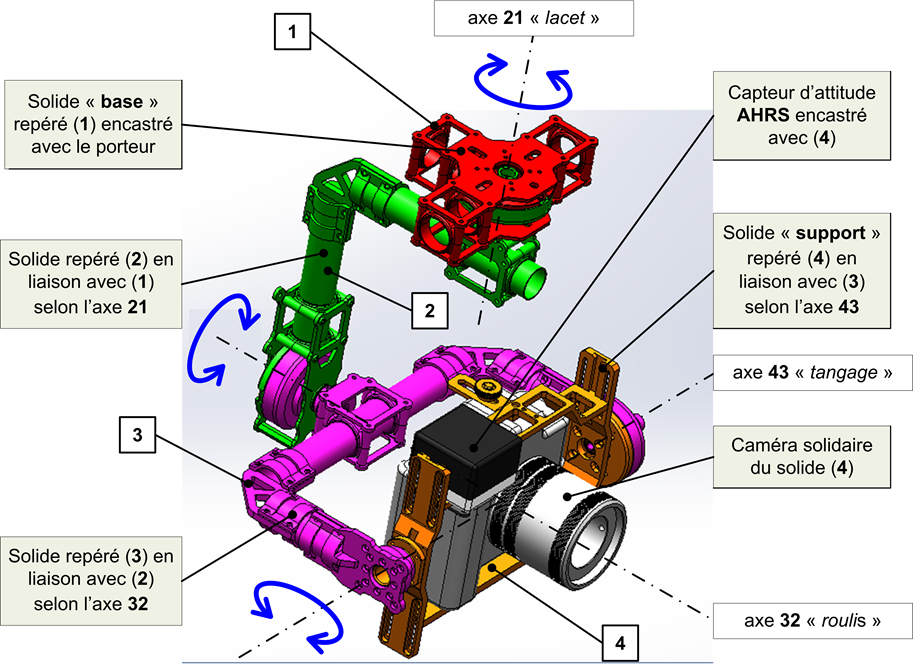
\includegraphics[width=.75\linewidth]{fig_00}
}%figues de la page de garde

\def\xxtitreexo{RobuROC 6 : Plate-forme d'exploration tout terrain}
\def\xxsourceexo{\hspace{.2cm} \footnotesize{\textsl{CCMP PSI 2009}}}


\iflivret
\pagestyle{empty}


%%%%%%%% PAGE DE GARDE COURS
\ifcours
\begin{tikzpicture}[remember picture,overlay]
\node at (current page.north west)
{\begin{tikzpicture}[remember picture,overlay]
\node[anchor=north west,inner sep=0pt] at (0,0) {\includegraphics[width=\paperwidth]{\thechapterimage}};
\draw[anchor=west] (-2cm,-8cm) node [line width=2pt,rounded corners=15pt,draw=ocre,fill=white,fill opacity=0.6,inner sep=40pt]{\strut\makebox[22cm]{}};
\draw[anchor=west] (1cm,-8cm) node {\huge\sffamily\bfseries\color{black} %
\begin{minipage}{1cm}
\rotatebox{90}{\LARGE\sffamily\textsc{\color{ocre}\textbf{\xxnumpartie}}}
\end{minipage} \hfill
\begin{minipage}[c]{14cm}
\begin{titrepartie}
\begin{flushright}
\renewcommand{\baselinestretch}{1.1} 
\Large\sffamily\textsc{\textbf{\xxpartie}}
\renewcommand{\baselinestretch}{1} 
\end{flushright}
\end{titrepartie}
\end{minipage} \hfill
\begin{minipage}[c]{3.5cm}
{\large\sffamily\textsc{\textbf{\color{ocre} \discipline}}}
\end{minipage} 
 };
\end{tikzpicture}};
\end{tikzpicture}


\begin{tikzpicture}[overlay]
\node[shape=rectangle, 
      rounded corners = .25 cm,
	  draw= ocre,
	  line width=2pt, 
	  fill = ocre!10,
	  minimum width  = 2.5cm,
	  minimum height = 3cm,] at (18cm,0) {};
\node at (17.7cm,0) {\rotatebox{90}{\textbf{\Large\color{ocre}{\classe}}}};
%{};
\end{tikzpicture}

\vspace{3.5cm}

\begin{tikzpicture}[remember picture,overlay]
\draw[anchor=west] (-2cm,-6cm) node {\huge\sffamily\bfseries\color{black} %
\begin{minipage}{2cm}
\begin{center}
\LARGE\sffamily\textsc{\color{ocre}\textbf{\xxactivite}}
\end{center}
\end{minipage} \hfill
\begin{minipage}[c]{15cm}
\begin{titrechapitre}
\renewcommand{\baselinestretch}{1.1} 
\Large\sffamily\textsc{\textbf{\xxnumchapitre}}

\Large\sffamily\textsc{\textbf{\xxchapitre}}
\vspace{.5cm}

\renewcommand{\baselinestretch}{1} 
\normalsize\normalfont
\xxcompetences
\end{titrechapitre}
\end{minipage}  };
\end{tikzpicture}
\vfill

\begin{flushright}
\begin{minipage}[c]{.3\linewidth}
\begin{center}
\xxfigures
\end{center}
\end{minipage}\hfill
\begin{minipage}[c]{.6\linewidth}
\startcontents
\printcontents{}{1}{}
\end{minipage}
\end{flushright}

\begin{tikzpicture}[remember picture,overlay]
\draw[anchor=west] (4.5cm,-.7cm) node {
\begin{minipage}[c]{.2\linewidth}
\begin{flushright}

\includegraphics[width=2cm]{logoCC}
\end{flushright}
\end{minipage}
\begin{minipage}[c]{.2\linewidth}
\textsl{\xxauteur} \\
\textsl{\classe}
\end{minipage}
 };
\end{tikzpicture}
\newpage
\pagestyle{fancy}

\newpage
\pagestyle{fancy}

\else
\fi


%%%%%%%% PAGE DE GARDE TD
\iftd
%\begin{tikzpicture}[remember picture,overlay]
%\node at (current page.north west)
%{\begin{tikzpicture}[remember picture,overlay]
%\draw[anchor=west] (-2cm,-3.25cm) node [line width=2pt,rounded corners=15pt,draw=ocre,fill=white,fill opacity=0.6,inner sep=40pt]{\strut\makebox[22cm]{}};
%\draw[anchor=west] (1cm,-3.25cm) node {\huge\sffamily\bfseries\color{black} %
%\begin{minipage}{1cm}
%\rotatebox{90}{\LARGE\sffamily\textsc{\color{ocre}\textbf{\xxnumpartie}}}
%\end{minipage} \hfill
%\begin{minipage}[c]{13.5cm}
%\begin{titrepartie}
%\begin{flushright}
%\renewcommand{\baselinestretch}{1.1} 
%\Large\sffamily\textsc{\textbf{\xxpartie}}
%\renewcommand{\baselinestretch}{1} 
%\end{flushright}
%\end{titrepartie}
%\end{minipage} \hfill
%\begin{minipage}[c]{3.5cm}
%{\large\sffamily\textsc{\textbf{\color{ocre} \discipline}}}
%\end{minipage} 
% };
%\end{tikzpicture}};
%\end{tikzpicture}

%%%%%%%%%% PAGE DE GARDE TD %%%%%%%%%%%%%%%
%\begin{tikzpicture}[overlay]
%\node[shape=rectangle, 
%      rounded corners = .25 cm,
%	  draw= ocre,
%	  line width=2pt, 
%	  fill = ocre!10,
%	  minimum width  = 2.5cm,
%	  minimum height = 2.5cm,] at (18.5cm,0) {};
%\node at (17.7cm,0) {\rotatebox{90}{\textbf{\Large\color{ocre}{\classe}}}};
%%{};
%\end{tikzpicture}

% PARTIE ET CHAPITRE
%\begin{tikzpicture}[remember picture,overlay]
%\draw[anchor=west] (-1cm,-2.1cm) node {\large\sffamily\bfseries\color{black} %
%\begin{minipage}[c]{15cm}
%\begin{flushleft}
%\xxnumchapitre \\
%\xxchapitre
%\end{flushleft}
%\end{minipage}  };
%\end{tikzpicture}

% Bandeau titre exo
\begin{tikzpicture}[remember picture,overlay]
\draw[anchor=west] (-2cm,-4cm) node {\huge\sffamily\bfseries\color{black} %
\begin{minipage}{5cm}
\begin{center}
\LARGE\sffamily\color{ocre}\textbf{\textsc{\xxactivite}}

\begin{center}
\xxfigures
\end{center}

\end{center}
\end{minipage} \hfill
\begin{minipage}[c]{12cm}
\begin{titrechapitre}
\renewcommand{\baselinestretch}{1.1} 
\large\sffamily\textbf{\textsc{\xxtitreexo}}

\small\sffamily{\textbf{\textit{\color{black!70}\xxsourceexo}}}
\vspace{.5cm}

\renewcommand{\baselinestretch}{1} 
\normalsize\normalfont
\xxcompetences
\end{titrechapitre}
\end{minipage}  };
\end{tikzpicture}

\else
\fi


%%%%%%%% PAGE DE GARDE FICHE
\iffiche
\begin{tikzpicture}[remember picture,overlay]
\node at (current page.north west)
{\begin{tikzpicture}[remember picture,overlay]
\draw[anchor=west] (-2cm,-3.25cm) node [line width=2pt,rounded corners=15pt,draw=ocre,fill=white,fill opacity=0.6,inner sep=40pt]{\strut\makebox[22cm]{}};
\draw[anchor=west] (1cm,-3.25cm) node {\huge\sffamily\bfseries\color{black} %
\begin{minipage}{1cm}
\rotatebox{90}{\LARGE\sffamily\textsc{\color{ocre}\textbf{\xxnumpartie}}}
\end{minipage} \hfill
\begin{minipage}[c]{14cm}
\begin{titrepartie}
\begin{flushright}
\renewcommand{\baselinestretch}{1.1} 
\large\sffamily\textsc{\textbf{\xxpartie} \\} 

\vspace{.2cm}

\normalsize\sffamily\textsc{\textbf{\xxnumchapitre -- \xxchapitre}}
\renewcommand{\baselinestretch}{1} 
\end{flushright}
\end{titrepartie}
\end{minipage} \hfill
\begin{minipage}[c]{3.5cm}
{\large\sffamily\textsc{\textbf{\color{ocre} \discipline}}}
\end{minipage} 
 };
\end{tikzpicture}};
\end{tikzpicture}


\begin{tikzpicture}[overlay]
\node[shape=rectangle, 
      rounded corners = .25 cm,
	  draw= ocre,
	  line width=2pt, 
	  fill = ocre!10,
	  minimum width  = 2.5cm,
	  minimum height = 2.5cm,] at (18.5cm,0.5cm) {};
%	  minimum height = 2.5cm,] at (18.5cm,0cm) {};
\node at (17.7cm,0.5) {\rotatebox{90}{\textsf{\textbf{\large\color{ocre}{\classe}}}}};
%{};
\end{tikzpicture}



\else
\fi



\else
\pagestyle{empty}


%%%%%%%% PAGE DE GARDE COURS
\ifcours
\begin{tikzpicture}[remember picture,overlay]
\node at (current page.north west)
{\begin{tikzpicture}[remember picture,overlay]
\node[anchor=north west,inner sep=0pt] at (0,0) {\includegraphics[width=\paperwidth]{\thechapterimage}};
\draw[anchor=west] (-2cm,-8cm) node [line width=2pt,rounded corners=15pt,draw=ocre,fill=white,fill opacity=0.6,inner sep=40pt]{\strut\makebox[22cm]{}};
\draw[anchor=west] (1cm,-8cm) node {\huge\sffamily\bfseries\color{black} %
\begin{minipage}{1cm}
\rotatebox{90}{\LARGE\sffamily\textsc{\color{ocre}\textbf{\xxnumpartie}}}
\end{minipage} \hfill
\begin{minipage}[c]{14cm}
\begin{titrepartie}
\begin{flushright}
\renewcommand{\baselinestretch}{1.1} 
\Large\sffamily\textsc{\textbf{\xxpartie}}
\renewcommand{\baselinestretch}{1} 
\end{flushright}
\end{titrepartie}
\end{minipage} \hfill
\begin{minipage}[c]{3.5cm}
{\large\sffamily\textsc{\textbf{\color{ocre} \discipline}}}
\end{minipage} 
 };
\end{tikzpicture}};
\end{tikzpicture}


\begin{tikzpicture}[overlay]
\node[shape=rectangle, 
      rounded corners = .25 cm,
	  draw= ocre,
	  line width=2pt, 
	  fill = ocre!10,
	  minimum width  = 2.5cm,
	  minimum height = 3cm,] at (18cm,0) {};
\node at (17.7cm,0) {\rotatebox{90}{\textbf{\Large\color{ocre}{\classe}}}};
%{};
\end{tikzpicture}

\vspace{3.5cm}

\begin{tikzpicture}[remember picture,overlay]
\draw[anchor=west] (-2cm,-6cm) node {\huge\sffamily\bfseries\color{black} %
\begin{minipage}{2cm}
\begin{center}
\LARGE\sffamily\textsc{\color{ocre}\textbf{\xxactivite}}
\end{center}
\end{minipage} \hfill
\begin{minipage}[c]{15cm}
\begin{titrechapitre}
\renewcommand{\baselinestretch}{1.1} 
\Large\sffamily\textsc{\textbf{\xxnumchapitre}}

\Large\sffamily\textsc{\textbf{\xxchapitre}}
\vspace{.5cm}

\renewcommand{\baselinestretch}{1} 
\normalsize\normalfont
\xxcompetences
\end{titrechapitre}
\end{minipage}  };
\end{tikzpicture}
\vfill

\begin{flushright}
\begin{minipage}[c]{.3\linewidth}
\begin{center}
\xxfigures
\end{center}
\end{minipage}\hfill
\begin{minipage}[c]{.6\linewidth}
\startcontents
\printcontents{}{1}{}
\end{minipage}
\end{flushright}

\begin{tikzpicture}[remember picture,overlay]
\draw[anchor=west] (4.5cm,-.7cm) node {
\begin{minipage}[c]{.2\linewidth}
\begin{flushright}

\includegraphics[width=2cm]{logoCC}
\end{flushright}
\end{minipage}
\begin{minipage}[c]{.2\linewidth}
\textsl{\xxauteur} \\
\textsl{\classe}
\end{minipage}
 };
\end{tikzpicture}
\newpage
\pagestyle{fancy}

\newpage
\pagestyle{fancy}

\else
\fi


%%%%%%%% PAGE DE GARDE TD
\iftd
%\begin{tikzpicture}[remember picture,overlay]
%\node at (current page.north west)
%{\begin{tikzpicture}[remember picture,overlay]
%\draw[anchor=west] (-2cm,-3.25cm) node [line width=2pt,rounded corners=15pt,draw=ocre,fill=white,fill opacity=0.6,inner sep=40pt]{\strut\makebox[22cm]{}};
%\draw[anchor=west] (1cm,-3.25cm) node {\huge\sffamily\bfseries\color{black} %
%\begin{minipage}{1cm}
%\rotatebox{90}{\LARGE\sffamily\textsc{\color{ocre}\textbf{\xxnumpartie}}}
%\end{minipage} \hfill
%\begin{minipage}[c]{13.5cm}
%\begin{titrepartie}
%\begin{flushright}
%\renewcommand{\baselinestretch}{1.1} 
%\Large\sffamily\textsc{\textbf{\xxpartie}}
%\renewcommand{\baselinestretch}{1} 
%\end{flushright}
%\end{titrepartie}
%\end{minipage} \hfill
%\begin{minipage}[c]{3.5cm}
%{\large\sffamily\textsc{\textbf{\color{ocre} \discipline}}}
%\end{minipage} 
% };
%\end{tikzpicture}};
%\end{tikzpicture}

%%%%%%%%%% PAGE DE GARDE TD %%%%%%%%%%%%%%%
%\begin{tikzpicture}[overlay]
%\node[shape=rectangle, 
%      rounded corners = .25 cm,
%	  draw= ocre,
%	  line width=2pt, 
%	  fill = ocre!10,
%	  minimum width  = 2.5cm,
%	  minimum height = 2.5cm,] at (18.5cm,0) {};
%\node at (17.7cm,0) {\rotatebox{90}{\textbf{\Large\color{ocre}{\classe}}}};
%%{};
%\end{tikzpicture}

% PARTIE ET CHAPITRE
%\begin{tikzpicture}[remember picture,overlay]
%\draw[anchor=west] (-1cm,-2.1cm) node {\large\sffamily\bfseries\color{black} %
%\begin{minipage}[c]{15cm}
%\begin{flushleft}
%\xxnumchapitre \\
%\xxchapitre
%\end{flushleft}
%\end{minipage}  };
%\end{tikzpicture}

% Bandeau titre exo
\begin{tikzpicture}[remember picture,overlay]
\draw[anchor=west] (-2cm,-4cm) node {\huge\sffamily\bfseries\color{black} %
\begin{minipage}{5cm}
\begin{center}
\LARGE\sffamily\color{ocre}\textbf{\textsc{\xxactivite}}

\begin{center}
\xxfigures
\end{center}

\end{center}
\end{minipage} \hfill
\begin{minipage}[c]{12cm}
\begin{titrechapitre}
\renewcommand{\baselinestretch}{1.1} 
\large\sffamily\textbf{\textsc{\xxtitreexo}}

\small\sffamily{\textbf{\textit{\color{black!70}\xxsourceexo}}}
\vspace{.5cm}

\renewcommand{\baselinestretch}{1} 
\normalsize\normalfont
\xxcompetences
\end{titrechapitre}
\end{minipage}  };
\end{tikzpicture}

\else
\fi


%%%%%%%% PAGE DE GARDE FICHE
\iffiche
\begin{tikzpicture}[remember picture,overlay]
\node at (current page.north west)
{\begin{tikzpicture}[remember picture,overlay]
\draw[anchor=west] (-2cm,-3.25cm) node [line width=2pt,rounded corners=15pt,draw=ocre,fill=white,fill opacity=0.6,inner sep=40pt]{\strut\makebox[22cm]{}};
\draw[anchor=west] (1cm,-3.25cm) node {\huge\sffamily\bfseries\color{black} %
\begin{minipage}{1cm}
\rotatebox{90}{\LARGE\sffamily\textsc{\color{ocre}\textbf{\xxnumpartie}}}
\end{minipage} \hfill
\begin{minipage}[c]{14cm}
\begin{titrepartie}
\begin{flushright}
\renewcommand{\baselinestretch}{1.1} 
\large\sffamily\textsc{\textbf{\xxpartie} \\} 

\vspace{.2cm}

\normalsize\sffamily\textsc{\textbf{\xxnumchapitre -- \xxchapitre}}
\renewcommand{\baselinestretch}{1} 
\end{flushright}
\end{titrepartie}
\end{minipage} \hfill
\begin{minipage}[c]{3.5cm}
{\large\sffamily\textsc{\textbf{\color{ocre} \discipline}}}
\end{minipage} 
 };
\end{tikzpicture}};
\end{tikzpicture}


\begin{tikzpicture}[overlay]
\node[shape=rectangle, 
      rounded corners = .25 cm,
	  draw= ocre,
	  line width=2pt, 
	  fill = ocre!10,
	  minimum width  = 2.5cm,
	  minimum height = 2.5cm,] at (18.5cm,0.5cm) {};
%	  minimum height = 2.5cm,] at (18.5cm,0cm) {};
\node at (17.7cm,0.5) {\rotatebox{90}{\textsf{\textbf{\large\color{ocre}{\classe}}}}};
%{};
\end{tikzpicture}



\else
\fi



\fi
\setlength{\columnseprule}{.1pt}

\pagestyle{fancy}
\thispagestyle{plain}


\vspace{4.5cm}

\def\columnseprulecolor{\color{ocre}}
\setlength{\columnseprule}{0.4pt} 

%%%%%%%%%%%%%%%%%%%%%%%



\begin{multicols}{2}
\setcounter{exo}{0}
\subsection*{Présentation}

Les déplacements de la plate-forme sont contrôlés de la manière suivante :
\begin{itemize}
\item au niveau de chacun des 6 moteurs, des boucles de vitesse assurent l’asservissement dit « bas niveau » ;
\item à partir d’informations sur la position absolue de la plate-forme via le système GPS par exemple, un
asservissement en position de la plate-forme peut être mis en place (asservissement dit « haut niveau »).
\end{itemize}

\begin{obj}
Déterminer les paramètres de réglage de chacune des boucles d’asservissement en vitesse de la plate-forme par rapport au sol.
\end{obj}

\subsection*{Hypothèses et modélisation}
Afin de régler l’asservissement en vitesse de la plate-forme par rapport au sol :
\begin{itemize}
\item un déplacement en ligne droite de la plate-forme est considéré (consigne de vitesse $V_C(t)$, les paramètres
angulaires de lacet, tangage et roulis restent nuls) ;
le contact entre chaque pneumatique et le sol est considéré avec roulement sans glissement ;
\item pour la modélisation du fonctionnement des moteurs, nous supposerons une équi-répartition de la charge
extérieure sur chacun des six moteurs. Ainsi, pour une vitesse $V(t)$ de la plate-forme, les six moteurs tourneront à
la même vitesse $\Omega_{\text{Mot}}(t)$. Ils seront alimentés par une même tension de commande $U(t)$ et devront fournir un même couple moteur $C_{\text{Mot}}(t)$;
\item les efforts de perturbations (action mécanique de la pesanteur sur une pente…) seront répartis sur chacun des
axes des six moteurs et seront donc modélisés par un même couple de perturbation équivalent $C_{\text{equ}}(t)$ appliqué
sur chacun des axes moteurs ;
\item les caractéristiques inertielles de la plate-forme seront représentées au niveau de chaque axe moteur par un
moment d’inertie équivalent $\dfrac{J_{\text{eq}}}{6}$;
\item le comportement individuel d’un des six moteurs peut donc être approché par celui d’un moteur à courant continu
avec les équations électromécaniques suivantes : $U(t)=E(t)+rI(t)+L\dfrac{\dd I(t)}{\dd t}$ (équation électrique), 
$\dfrac{J_{\text{eq}}}{6} \dfrac{\dd \Omega_{\text{Mot}}(t)}{\dd t}=C_{\text{Mot}}(t)-C_{\text{equ}}(t)$ (équation mécanique), $E(t)=k_e \Omega_{\text{Mot}}(t)$ et $C_{\text{Mot}}(t)=k_cI(t)$ (équations de couplage).
\end{itemize}

\begin{center}
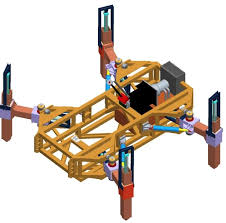
\includegraphics[width=\linewidth]{fig_01}
\end{center}


\subsection*{Description de l’asservissement en vitesse de la plate-forme par rapport au sol}
Pour une vitesse de consigne $V_C(t)$ [m/s], les microcontrôleurs de pilotage génèrent une vitesse de rotation de
consigne à appliquer à chaque moteur $\Omega_{C_{\text{Mot}}}(t)$ [rad/s] qui est convertie en une tension de consigne 
$U_C(t)$ [V]. Un capteur de vitesse monté sur l’axe de chaque moteur fournit une tension mesurée $U_m(t)$ [V], image de la vitesse de
rotation réelle $\Omega_{{\text{Mot}}}(t)$ . Un correcteur (défini par la suite) adapte le signal écart entre la tension de consigne et la tension mesurée, ce qui permet après amplification de définir la tension d’alimentation $U(t)$ à appliquer aux moteurs. La vitesse réelle de la plate-forme $V(t)$ est déterminée à partir de $\Omega_{{\text{Mot}}}(t)$ en l’absence de glissement.

\begin{center}
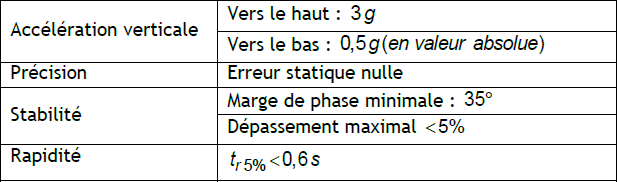
\includegraphics[width=\linewidth]{fig_02}
\end{center}

\begin{center}
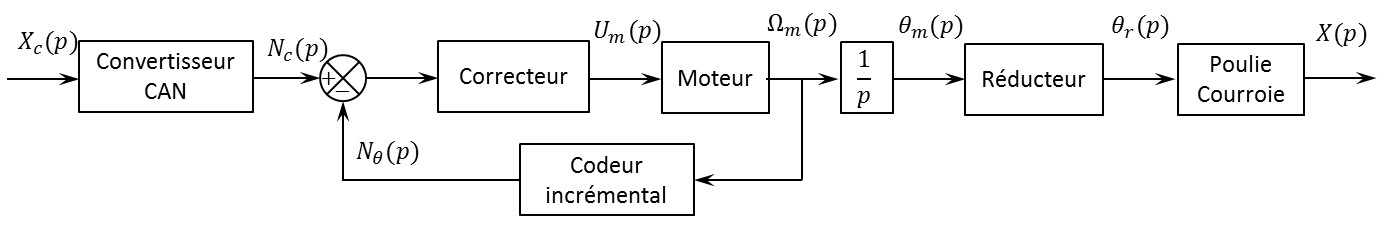
\includegraphics[width=\linewidth]{fig_03}
\end{center}

\begin{center}
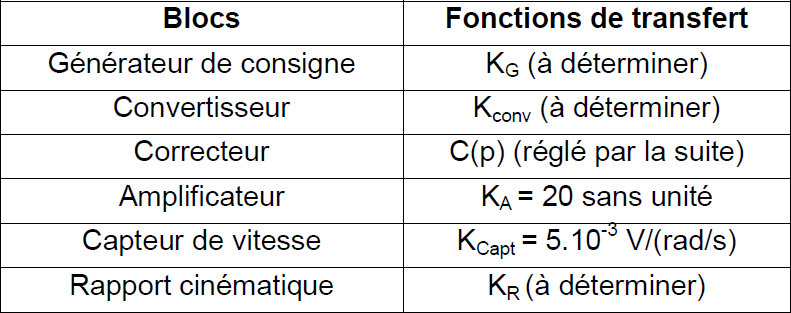
\includegraphics[width=\linewidth]{fig_04}
\end{center}

\subsection*{Cahier des charges à respecter}
\begin{center}
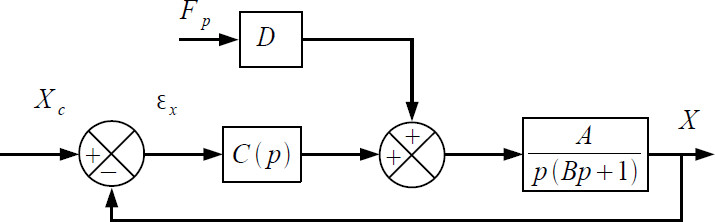
\includegraphics[width=\linewidth]{fig_05}
\end{center}


\subparagraph{}\textit{Déterminer les valeurs numériques et unités des gains associés au générateur de consigne (noté $K_G$), au rapport cinématique ($K_R$) et au convertisseur ($K_{\text{conv}}$) en sachant, que lorsque la vitesse réelle de la plateforme $V(t)$ est égale à la vitesse de consigne de la plate-forme $V_C(t)$, l’écart $\varepsilon(t)$ doit être nul.}
\ifprof
\begin{corrige}
\end{corrige}
\else
\fi


\subparagraph{}\textit{Compléter le schéma-blocs en y faisant figurer les fonctions de
transfert sous forme littérale dans le domaine de Laplace avec des conditions initiales nulles, ainsi que les
signes des sommateurs.}
\ifprof
\begin{corrige}
\end{corrige}
\else
\fi

\begin{center}
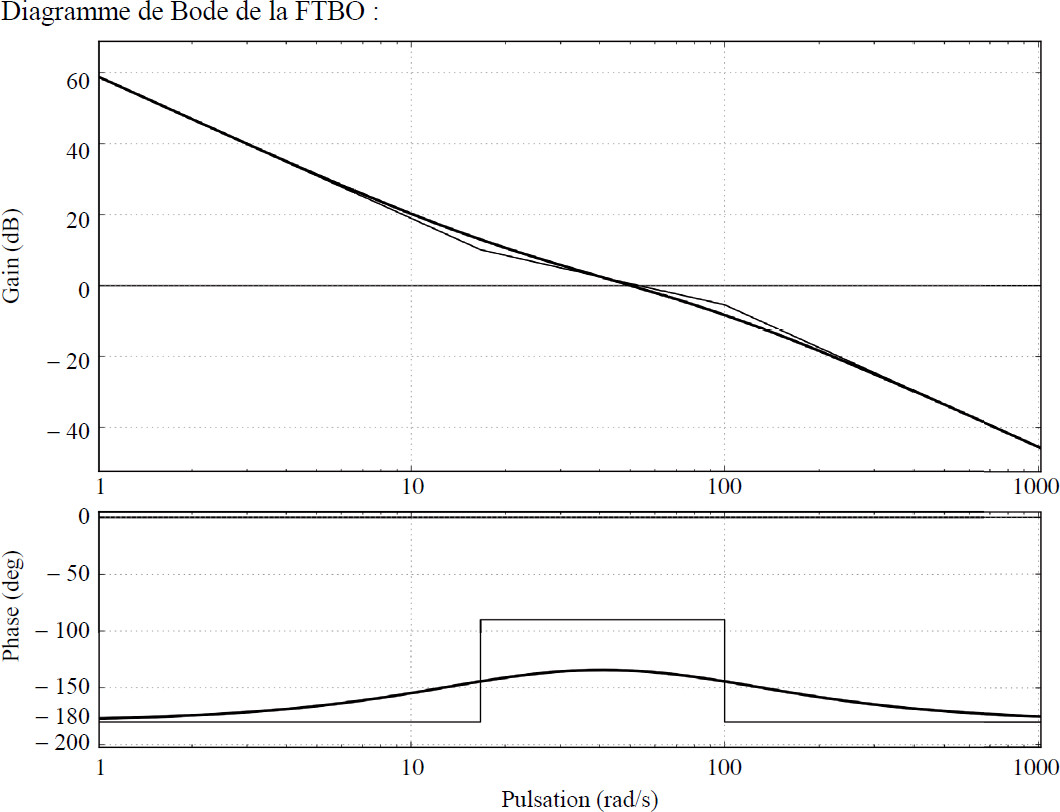
\includegraphics[width=\linewidth]{fig_06}
\end{center}

À partir de la modélisation des blocs, un schéma bloc à retour unitaire est tracé.

\begin{center}
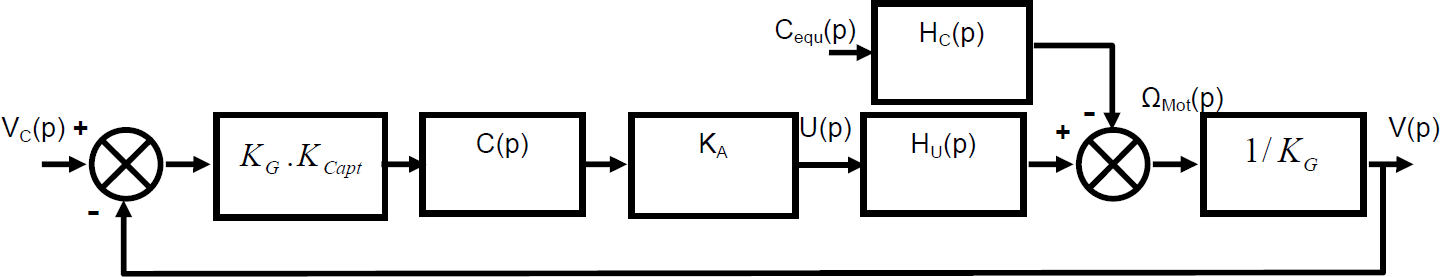
\includegraphics[width=\linewidth]{fig_07}
\end{center}

$H_U( p)$ et $H_C( p)$ sont les fonctions de transfert caractéristiques d’un des six moteurs. Nous retiendrons :
$H_U( p) = \dfrac{K_U}{\left( 1+T_1 p\right)\left( 1+T_2 p\right)}$ et $H_C( p)= \dfrac{K_C\left(1+\dfrac{L}{r}p \right)}{\left( 1+T_1 p\right)\left( 1+T_2 p\right)}$ avec 
$K_U = \SI{8,3}{rad.s^{-1}.V^{-1}}$, 
$K_C = \SI{152,7}{rad.s^{-1}.N^{-1}.m^{-1}}$, 
$T_1 = \SI{2,1}{ms}$ et $T_2 = \SI{0,36}{s}$.

\subsection*{Étude des performances sans correction : $C( p) =1$}

Nous distinguerons dans la suite :
\begin{itemize}
\item l’étude en poursuite : le couple de perturbation équivalent $C_{\text{equ}} (t)$ est nul. $V_c(t)$ varie;
\item l’étude en régulation : la vitesse de consigne de la plate-forme $V_c (t)$ est nulle. $C_{\text{equ}} (t)$ varie.
\end{itemize}
Les diagrammes de Bode de la Fonction de Transfert en Boucle Ouverte $\text{FTBO}(p)$ non corrigée sont fournis ci-dessous pour $C( p) = 1$.


\begin{center}
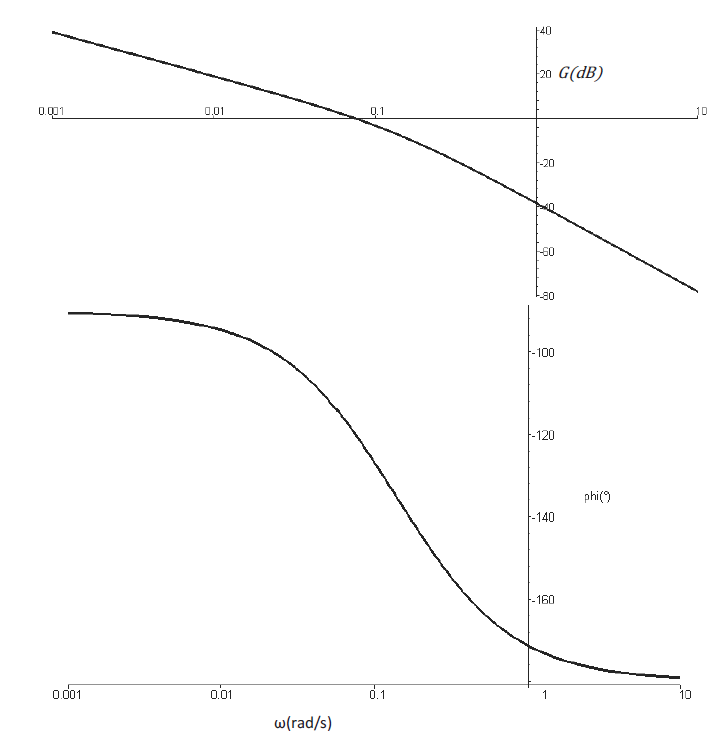
\includegraphics[width=\linewidth]{fig_08}
\end{center}


\subparagraph{}\textit{Le système étudié est-il stable théoriquement ? Justifier vos réponses.}
\ifprof
\begin{corrige}
\end{corrige}
\else
\fi


\subparagraph{}\textit{Étudier l’aptitude du système sans correction à respecter les critères de précision. Vous déterminerez
notamment les expressions littérales de l’erreur statique en poursuite pour une consigne de vitesse de la
plate-forme $V_c(t)$ en échelon d’amplitude $V_{CO}$ : $V_c(t)=V_{CO}u(t)$ (avec $u(t)$ l’échelon unitaire) et de
l’influence en régulation d’une perturbation $C_{\text{equ}}(t)$ en échelon d’amplitude $C_0$, sur la vitesse réelle $V(t)$ de
la plate-forme en régime permanent.}
\ifprof
\begin{corrige}
\end{corrige}
\else
\fi

\subsection*{Étude des performances avec un correcteur de fonction de transfert $C(p)=\dfrac{K_I}{p}$}

\subparagraph{}\textit{Indiquer quelle est la nature de la correction effectuée par ce correcteur (ou désignation du correcteur) ? Indiquer pour quelle(s) raison(s) principale(s) ce correcteur a été choisi. Valider ce choix vis à vis du cahier
des charges. Sans calcul, donner l’influence de ce correcteur sur les autres performances attendues.}
\ifprof
\begin{corrige}
\end{corrige}
\else
\fi

Reprenons le diagramme de Bode de la Fonction de Transfert en Boucle Ouverte $\text{FTBO}( p)$ non corrigée

\subparagraph{}\textit{Tracer les diagrammes de Bode du correcteur avec $K_I = \SI{1}{s^{-1}}$. Déterminer alors la valeur de $K_I$ maximale notée $K_{I\text{ max}}$ permettant de respecter les marges de stabilité énoncées dans le cahier des charges.}
\ifprof
\begin{corrige}
\end{corrige}
\else
\fi

Afin d’évaluer analytiquement le temps de réponse à 5\%, il est proposé d’adopter une modélisation simplifiée du
comportement du moteur en conservant uniquement le mode associé au pôle «~dominant~». On donne $T_{5\% \text{mini}} \omega_0 = 3$ avec $\omega_0$ la pulsation propre non amortie d’un système fondamental du second ordre.


\subparagraph{}\textit{En analysant les valeurs numériques des pôles de la fonction de transfert du moteur en poursuite $H_U(p)$,
préciser quel est le pôle dominant et proposer alors un modèle simplifié de la fonction de transfert $H_U(p)$.
Déterminer alors la valeur numérique de $K_I$ notée $K_{I 5\%}$ minimisant le temps de réponse à 5\% pour une
entrée échelon en poursuite. Calculer alors la valeur approchée du temps de réponse à 5\% minimale $T_{5\% \text{mini}}$
et comparer la au cahier des charges.}
\ifprof
\begin{corrige}
\end{corrige}
\else
\fi

\subsection*{Étude des performances avec un correcteur proportionnel intégral $C(p)=K_P\left(1+\dfrac{1}{T_I p} \right)$}

Le correcteur est remplacé par un correcteur proportionnel intégral. Des réponses temporelles du système corrigé sont
tracées ci-dessous avec :
\begin{itemize}
\item une consigne de vitesse unitaire de la plate-forme $V_c(t)= u(t)$ (avec $u(t)$ l’échelon unitaire);
\item une perturbation sous la forme d’un échelon unitaire retardé de 5 secondes $C_{\text{equ}} (t) = u(t - 5)$;
\item un gain du correcteur $K_p = 1$;
\item différentes valeurs de $T_I$.
\end{itemize}


\begin{center}
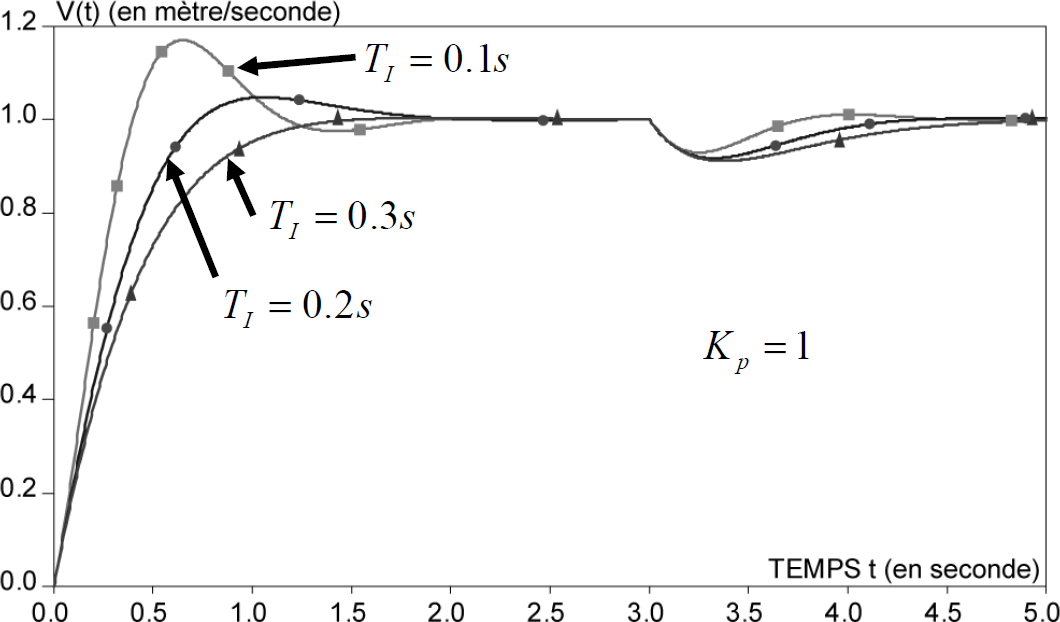
\includegraphics[width=\linewidth]{fig_09}
\end{center}

\subparagraph{}\textit{Parmi les différentes valeurs de $T_I$, choisir celle qui assure le temps de réponse à 5\% le plus faible.}
\ifprof
\begin{corrige}
\end{corrige}
\else
\fi

La valeur de $T_I$ déterminée à la question précédente est retenue pour le réglage du correcteur proportionnel intégral.
Il s’agit alors de choisir le gain du correcteur $K_p$ à partir des simulations proposées.

\subparagraph{}\textit{Parmi les différentes valeurs de $K_p$, choisir la valeur qui assure un temps de réponse à 5\% au plus près de la valeur fournie dans le cahier des charges.}
\ifprof
\begin{corrige}
\end{corrige}
\else
\fi
\begin{center}
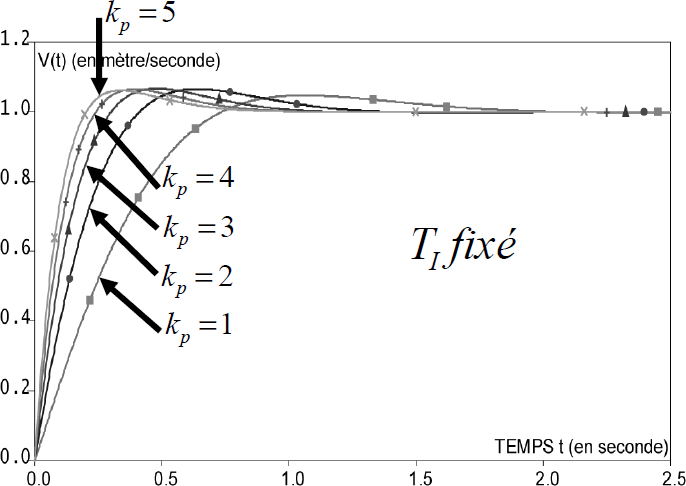
\includegraphics[width=\linewidth]{fig_10}
\end{center}

\begin{center}
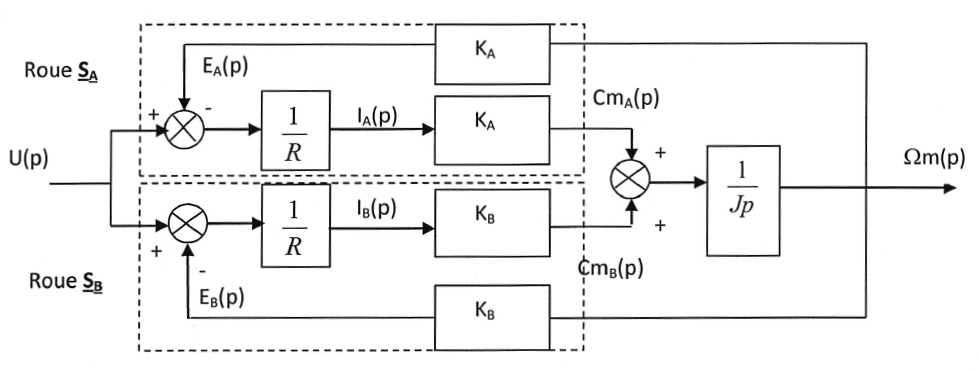
\includegraphics[width=\linewidth]{fig_11}
\end{center}
Avec le couple de valeurs ($T_I$ et $K_p$) obtenu, la réponse fréquentielle du système en boucle ouverte a été tracée sur la figure suivante.

\begin{center}
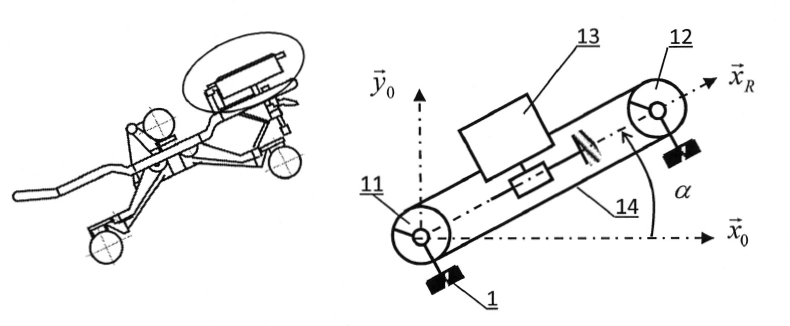
\includegraphics[width=\linewidth]{fig_12}
\end{center}


\subparagraph{}\textit{Conclure quant à la capacité de ce correcteur à respecter tous les critères du cahier des charges.}
\ifprof
\begin{corrige}
\end{corrige}
\else
\fi


%\begin{enumerate}
%\item $t_{5\%}\simeq \SI{0,61}{ s}$. 
%\end{enumerate}
\end{multicols}

%\end{document}
%
%\subparagraph{}\textit{}
%
%
%\begin{center}
%\includegraphics[width=\linewidth]{}
%\end{center}
%
%\begin{center}
%\includegraphics[width=\linewidth]{}
%\textit{}
%\end{center}
%
